\documentclass[main]{subfiles}
\begin{document}

%@@@@@@@@@@@@@@@@@@@@@@@@@@@@@@
% Main Topics: Introduction 06.12.2018
% Lecturer: Matthew Cook
% author: Vanessa Leite - base document from benelot/eth-intro-to-neuroinformatics-summary

\section{Perceptron Learning Algorithm}

\begin{itemize}[noitemsep,nolistsep]
	\item Choose random initial weights.
	\item Calculate output for given input.
	\item If the output is not the expected value, then $e=d-c$, where $d$ is the desired output and $c$ the current output.
	\item Change the weight of inputs and bias by $\Delta w_i=e\cdot\alpha\cdot x_i$. For the bias, always use $x=1$.
\end{itemize}

\section{Hopfield Networks}

\begin{itemize}[noitemsep,nolistsep]
	\item Every node is connected to every other node but not to itself.
	\item Connection weights are symmetric.
	\item $\sum x_iw_i < 0$ is disabled, $\sum x_iw_i \geq 0$ is enabled.
	\item Entire Network is in some state at any time. Set of active units of the entire network is important.
	\item Some states are stable and some are not. While in an unstable state, updating the network leads to a state change.
	\item Stable state is a local minimum. This does however not have to happen.
	\item Bias is an unit that is always on.
	\item Weight of a connection is correlated to frequency of firing together (Hebbian learning).
\end{itemize}

\subsection{Hopfield and Memory}
\begin{itemize}[noitemsep,nolistsep]
	\item A hopfield network is an associative type of memory. Information is stored in the stable states as local minima.
	\item It is important that information is distinct.
	\item Associative memory has room for error but is still recognizable. Convergence to nearby stable states.
	\item Only helpful if reliable input.
	\item If some units are retrievable and all others are set randomly, the correct units will eventually set wrong units right.
\end{itemize}

\subsection{Updates and State Dynamics}
\begin{itemize}[noitemsep,nolistsep]
	\item Nodes can be updated synchronously or asynchronously.
	\item State: Set of units that are active.
	\item Dynamics: Units update their activity level.
	\item When a node is updated, weights are considered from all other active nodes, like with a perceptron.
	\item Asynchronous updates (greedy algorithm) converge to a stable state (sequential), but the converged state can depend on update order.
	\item Asynchronous is either in max-clique state if activity is in $\{0,1\}$ or min-cut if activities are in $\{-1,1\}$.
	\item Synchronous, parallel updates either also go to a stable state, just like asynchronous, or can get stuck in a pair of patterns (flipping or cyclic).
\end{itemize}
\begin{figure}[H]
	\centering
	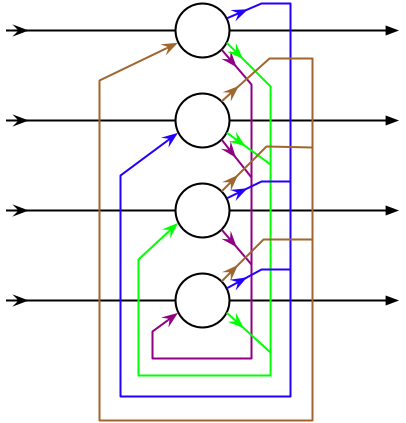
\includegraphics[width=0.3\textwidth]{hopfield-network.png}
\end{figure}



\end{document}
